\documentclass[ignorenonframetext,t]{beamer}

% \setbeameroption{show notes}
\usepackage[spanish]{babel}
\usepackage[T1]{fontenc}
\usepackage[utf8]{inputenc}
\usepackage[export]{adjustbox} % https://texblog.org/2014/02/20/figure-with-border-in-latex/
\usepackage{ulem}

\usepackage{pgfpages}
%\setbeameroption{show notes}
%\setbeameroption{show notes on second screen=right}

% 19.5x9 is alvherre's current phone aspect ratio
%\geometry{papersize={19.5cm,9cm}}
\IfFileExists{upquote.sty}{\usepackage{upquote}}{}

\usetheme{Frankfurt}
\setbeamertemplate{items}[circle] 
\beamertemplatenavigationsymbolsempty

% EDB colors
\definecolor{fiveninesnavy}{rgb}{0.07058,0.8627,0.2745}    % #121646
\definecolor{opensourceorange}{rgb}{1,0.243,0}           % #ff3e00

%\setbeamercolor{palette primary}{use={structure,normal text},bg=structure.bg, fg=normal text.fg!0!fiveninesnavy}


%\usecolortheme[RGB={18,22,70}]{structure}  % "five nines navy"
%\usecolortheme[RGB={255,62,00}]{structure}  % orange

\author{Álvaro Herrera\\
PostgreSQL developer}
\institute{\href{https://www.enterprisedb.com/}{
\includegraphics[width=1.4cm]{EDB_Logo- primary.png} \\ https://www.EnterpriseDB.com/}}
\date{Prague PostgreSQL Developer Day \\
February 2023}
% This puts logo at the right of the slide.
%\logo{\href{http://www.2ndquadrant.com/}{
\includegraphics[height=.4cm]{EDB_Logo- primary.png}}\hfill}
% Logo at the left corner:
\setbeamertemplate{footline}{%
  \hspace{0.3cm}%
  \href{https://www.enterprisedb.com/}{
\includegraphics[height=.4cm]{EDB_Logo- primary.png}}%
  \hfill\vspace{0.2cm}%
  }

%https://tex.stackexchange.com/questions/119277/non-bitmapped-thumb-up-symbol-for-flagging-good-practice-tips
\usepackage{fontawesome}

\usepackage{pmboxdraw}

\usepackage{listings}
\lstset{language=SQL,
basicstyle=\footnotesize\ttfamily,keywordstyle=\bfseries\color{green!40!black},%
columns=fullflexible, keepspaces, upquote,
morekeywords={with, merge, returning},
deletekeywords={YEAR},
showspaces=false,showstringspaces=false,
literate={á}{{\'{a}}}{1}
         {é}{{\'{e}}}{1}
         {í}{{\'{i}}}{1}
         {ó}{{\'{o}}}{1}
         {ú}{{\'{u}}}{1}
         {¡}{{!`}}{1}
         {┌}{{\textSFi}}1 
         {─}{{\textSFx}}1 
         {│}{{\pmboxdrawuni{2502}}}1
         {┬}{{\textSFvi}}1
         {┐}{{\textSFiii}}1
         {├}{{\textSFviii}}1
         {┼}{{\textSFv}}1
         {┤}{{\textSFix}}1
         {┴}{{\textSFvii}}1
         {└}{{\textSFii}}1
         {┘}{{\textSFiv}}1
%morekeywords={data,wrapper,library,language}%
}

\title{The MERGE Command}
\newcommand{\putcollection}{
  \put(0,50){
    \parbox{\textwidth}{
      \fontsize{30}{30}\selectfont
      Álvaro Herrera \\
      PostgreSQL developer \\
      EDB
    }
  }
}
\newcommand{\insertcopyright}{}
\renewcommand{\insertcopyright}{(C) EDB 2023}
%\date{}

% Make pauses show greyed-out future text
\setbeamercovered{transparent}

\begin{document}

\begin{frame}[plain]
  \titlepage
\end{frame}

\begin{frame}
  \frametitle{So what is MERGE anyway?}
  \begin{itemize}
    \item A ``new'' SQL DML command

  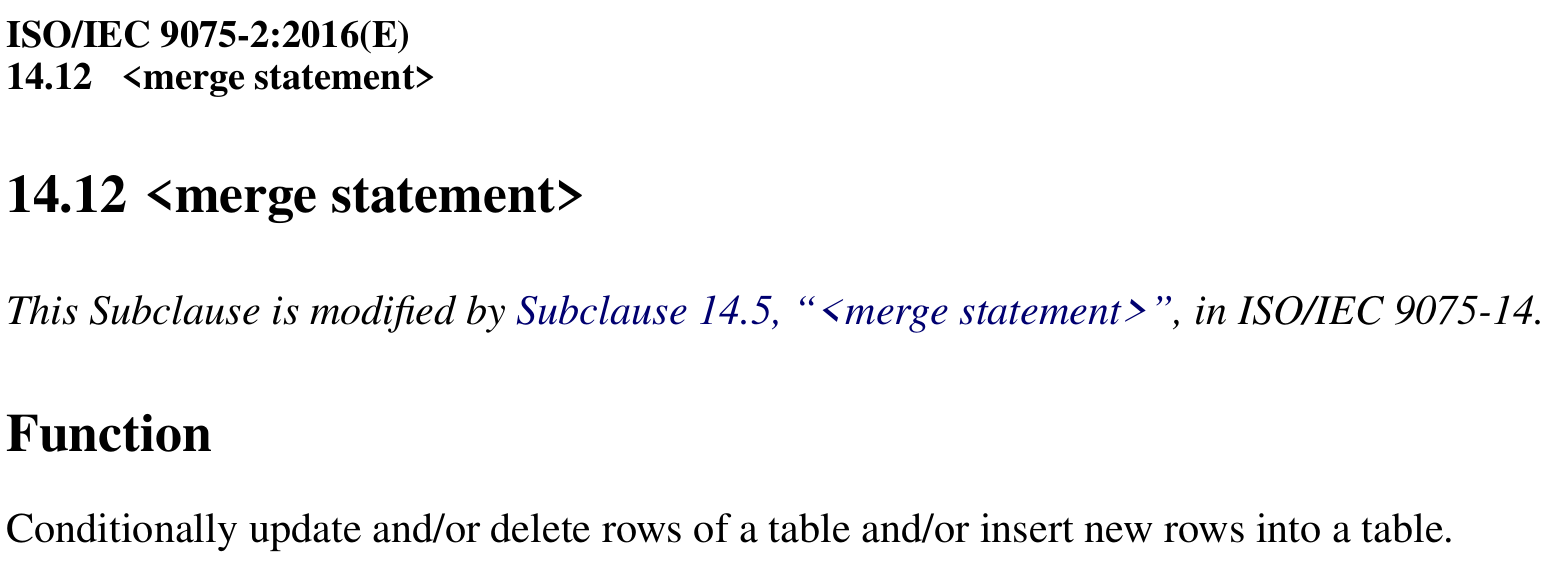
\includegraphics[width=0.7\paperwidth, frame]{sqlstd-merge.png}
  \end{itemize}


  \begin{itemize}
    \item Introduced in SQL:2003
  \pause
\item Is it UPSERT?
  \end{itemize}

\end{frame}
\note{Big discussion in pgsql-hackers community about whether MERGE would be useful for UPSERT; close study of concurrency considerations in the SQL standard led the community to opt for a separate command.  MERGE seemed more suited for batch-processing, OLAP style, rather than individual row processing OLTP-style.}

\begin{frame}[fragile]
  \frametitle{What MERGE is not}
  \begin{itemize}
    \item MERGE is not UPSERT
    \item (PostgreSQL ended up introducing non-standard INSERT~ON~CONFLICT~UPDATE in 9.5 (2016)
  \end{itemize}
% /*
% */ create table wines (winery text , brand text, variety text, year int, bottles int); /*
% */ alter table wines add unique (winery, brand, variety, year);

\begin{lstlisting}
 INSERT INTO wines (winery, brand, variety, year, bottles)
      VALUES ('Concha y Toro', 'Sunrise', 'Chardonnay', 2021, 96)
 ON CONFLICT (winery, brand, variety, year) DO
  UPDATE SET bottles = wines.bottles + EXCLUDED.bottles;
\end{lstlisting}

\pause
  \begin{itemize}
    \item \faThumbsOUp{} Special (index-)row locking is used
    \item \faThumbsOUp{} Fast and ``concurrency correct''
      \pause
    \item \faThumbsODown{} It can't do DELETE
    \item \faThumbsODown{} It is not standard and very different from MERGE
    \item \faThumbsODown{} Concurrency considerations are different
    \item<3> )
  \end{itemize}
\end{frame}

\note[itemize]{
\item I'll use this to introduce my sample data model
\item I come form Chile, which produces lots of wine
\item In this model, you import boxes of bottles of wine from Chile
\item You want to keep track of your inventory and shipment}

\begin{frame}
  \frametitle{MERGE history}
  \begin{itemize}
    \item First implementation attempt in PostgreSQL 11 (2018)
    \item Fully implemented in PostgreSQL 15 (2022)
    \item Other RDBMS systems have it
      \begin{itemize}
	\item Oracle\texttrademark{} 11 had it (2007?)
	\item SQL Server\texttrademark{} 2008 had it
      \end{itemize}
      \pause
    \item ... so Postgres having it, improves chances of migration
    \begin{itemize} \item (even though there are still some differences) \end{itemize}
  \end{itemize}
\end{frame}


\begin{frame}[fragile]
  \frametitle{MERGE example}

  \begin{lstlisting}
CREATE TABLE wines (winery text, brand text, variety text, year int,
                    bottles int);
ALTER TABLE wines ADD UNIQUE (winery, brand, variety, year);
CREATE TABLE shipment (LIKE wines);

INSERT INTO shipment VALUES
       ('Concha y Toro', 'Sunrise', 'Chardonnay', 2021, 96),
       ('Concha y Toro', 'Sunrise', 'Merlot', 2022, 120),
       ('Concha y Toro', 'Marqués de Casa y Concha', 'Carmenere',
                         2021, 48),
       ('Concha y Toro', 'Casillero del Diablo', 'Cabernet Sauvignon',
                         2019, 240);
\end{lstlisting}
\end{frame}

\begin{frame}[fragile]
  \frametitle{MERGE example}

  \begin{lstlisting}[basicstyle=\tiny]
CREATE TABLE wines (winery text, brand text, variety text, year int, bottles int);
CREATE TABLE shipment (LIKE wines);
\end{lstlisting}

\begin{lstlisting}
MERGE INTO wines AS w
     USING shipment AS s
        ON (w.winery, w.brand, w.variety, w.year) =
           (s.winery, s.brand, s.variety, s.year)

WHEN MATCHED THEN
     UPDATE SET bottles = w.bottles + s.bottles

WHEN NOT MATCHED THEN
     INSERT (winery, brand, variety, year, bottles)
     VALUES (s.winery, s.brand, s.variety, s.year, s.bottles);
\end{lstlisting}
\end{frame}

\note[itemize]{
\item Parts of the command:
  \begin{itemize}
    \item Target table
    \item Source ``table''
    \item WHEN MATCHED / NOT MATCHED clauses
    \item UPDATE/DELETE do not have WHERE; INSERT does not have INTO
    \item WHEN NOT MATCHED only references columns in source
  \end{itemize}
\item Execution:
  \begin{itemize}
    \item The target and source tables are joined
    \item WHEN [NOT] MATCHED clauses are evaluated for each row of the join
    \item If any NOT MATCHED exist, we use a LEFT JOIN
    \item If no NOT MATCHED, we don't need those rows; a normal (inner) join is used
  \end{itemize}

}

\begin{frame}[fragile]
  \frametitle{MERGE syntax}

  \begin{lstlisting}
  [ WITH clause ]

    MERGE INTO target_table
         USING { source table or query }
            ON { join condition }

     WHEN MATCHED [ AND expression ] THEN
         UPDATE SET { columns / values }

     WHEN MATCHED [ AND expression ] THEN
         DELETE
     
     WHEN NOT MATCHED [ AND expression ] THEN
         INSERT { columns / values }
     ;
  \end{lstlisting}

\end{frame}

\begin{frame}[fragile]
  \frametitle{Multiple WHEN-clause example}

  \begin{lstlisting}
  MERGE INTO wines w
       USING shipment s
          ON (w.winery, ...) = (s.winery, ...)

   WHEN MATCHED AND (w.bottles + s.bottles) <= 0
       DELETE
   WHEN MATCHED AND (w.bottles + s.bottles) > 1200
       UPDATE SET on_sale = true, bottles = w.bottles+s.bottles
   WHEN MATCHED AND (w.bottles + s.bottles) < 120
       UPDATE SET on_sale = false, bottles = w.bottles+s.bottles
   WHEN MATCHED
       UPDATE SET bottles = w.bottles + s.bottles
   WHEN NOT MATCHED AND s.bottles < 12 THEN
       DO NOTHING
   WHEN NOT MATCHED THEN
       INSERT ( ... ) VALUES ( ... )
  \end{lstlisting}
\end{frame}
\note[itemize]{
\item The first WHEN [NOT] MATCHED is run for each tuple
\item Relative order of all WHEN MATCHED and all WHEN NOT MATCHED is critical
\item Order of WHEN MATCH is irrelevant relateive to WHEN NOT MATCHED
\item Tuples updated concurrently are re-evaluated to see if new copy
  still matches the conditions of the clause being executed; if not, search
  restarts from the top
\item WHEN MATCHED can change into WHEN NOT MATCHED
\item WHEN NOT MATCHED does not change into WHEN MATCHED
\item Concurrent insert can cause command to error
}

\begin{frame}
  \frametitle{Dealing with concurrency}
  \begin{itemize}
    \item Easiest is to not run two MERGEs concurrently targetting the same table
      \begin{itemize}
	\item (perhaps: \texttt{LOCK TABLE wines IN SHARE MODE})
      \end{itemize}
    \item If you must have two, make them not have WHEN~NOT~MATCHED~THEN~INSERT clauses
    \item If you must allow concurrent insertion, rewrite to INSERT~ON~CONFLICT~UPDATE
      \pause
    \item If you do not lock the table, test extensively for concurrent scenarios
      \begin{itemize}
	\item plan to spend \sout{at least twice as long} much longer testing than developing
      \end{itemize}
  \end{itemize}
\end{frame}

\begin{frame}[fragile]
  \frametitle{Duplicates in MERGE source}

  What if my source table has ``duplicates''?

  \pause
  \begin{verbatim}
-- update
ERROR:  MERGE command cannot affect row a second time

-- insert
ERROR:  duplicate key value violates unique constraint "wines_winery_brand_variety_year_key"
DETAIL:  Key (winery, brand, variety, year)=(Concha y Toro, Sunrise, Chardonnay, 2021) already exists.
\end{verbatim}
\end{frame}

\begin{frame}[fragile]
  \frametitle{Duplicates in MERGE source (2)}
  \begin{lstlisting}
  MERGE INTO wines AS w
       USING (   SELECT winery, brand, variety, year,
                        sum(bottles) as bottles
                   FROM shipment
               GROUP BY winery, brand, variety, year
	     ) AS s
          ON (w.winery, w.brand, w.variety, w.year) =
             (s.winery, s.brand, s.variety, s.year)
  WHEN MATCHED THEN
        UPDATE SET bottles = w.bottles + s.bottles
  WHEN NOT MATCHED THEN
        INSERT (winery, brand, variety, year, bottles)
        VALUES (s.winery, s.brand, s.variety, s.year, s.bottles)
  ;
  \end{lstlisting}	
\end{frame}

\begin{frame}[fragile]
  \frametitle{MERGE example 3}

  What if I run MERGE twice with the same source?
  \pause
  \begin{lstlisting}
ALTER TABLE shipment ADD COLUMN marked timestamp with time zone;
  \end{lstlisting}
\pause
  \begin{lstlisting}
WITH unmarked_shipment AS
 (UPDATE shipment SET marked = now() WHERE marked IS NULL
         RETURNING winery, brand, variety, year, bottles)

MERGE INTO wines AS w
     USING unmarked_shipment AS s
        ON (w.winery, w.brand, w.variety, w.year) =
           (s.winery, s.brand, s.variety, s.year)
WHEN MATCHED THEN
     UPDATE SET bottles = w.bottles + s.bottles

WHEN NOT MATCHED THEN
     INSERT (winery, brand, variety, year, bottles)
     VALUES (s.winery, s.brand, s.variety, s.year, s.bottles);
  \end{lstlisting}
\end{frame}

\begin{frame}[fragile]
  \frametitle{Combining both examples}

  \begin{lstlisting}
WITH unmarked_shipment AS
 (UPDATE shipment SET marked = now() WHERE marked IS NULL
         RETURNING winery, brand, variety, year, bottles)
MERGE INTO wines AS w
     USING (SELECT winery, brand, variety, year,
                        sum(bottles) as bottles
                   FROM unmarked_shipment
               GROUP BY winery, brand, variety, year) AS s
        ON (w.winery, w.brand, w.variety, w.year) =
           (s.winery, s.brand, s.variety, s.year)
WHEN MATCHED THEN
     UPDATE SET bottles = w.bottles + s.bottles
WHEN NOT MATCHED THEN
     INSERT (winery, brand, variety, year, bottles)
     VALUES (s.winery, s.brand, s.variety, s.year, s.bottles)
;
  \end{lstlisting}
\end{frame}

\begin{frame}
  \frametitle{Trigger behavior}

  \begin{itemize}
    \item Boring (it behaves as you'd expect)
      \begin{itemize}
	\item BEFORE EACH STATEMENT
	  \begin{itemize}
	    \item INSERT
	    \item UPDATE
	    \item DELETE
	  \end{itemize}
	\item BEFORE EACH ROW
	\begin{itemize} \item Each row as scanned by the join
	\end{itemize}
      \item AFTER EACH ROW
      \begin{itemize} \item Each row in the same order as above \end{itemize}
	  \item AFTER EACH STATEMENT
	    \begin{itemize}
	      \item DELETE
	      \item UPDATE
	      \item INSERT
	    \end{itemize}
      \end{itemize}
  \end{itemize}
\end{frame}

\begin{frame}[fragile]
  \frametitle{FOR STATEMENT triggers -- transition table example}

  \begin{lstlisting}
CREATE TABLE wine_audit (op varchar(1), datetime timestamptz,
			 oldrow jsonb, newrow jsonb);

CREATE FUNCTION wine_audit() RETURNS trigger LANGUAGE plpgsql AS $$
  BEGIN
    IF (TG_OP = 'DELETE') THEN
      INSERT INTO wine_audit
           SELECT 'D', now(), row_to_json(o), NULL FROM old_table o;
    ELSIF (TG_OP = 'INSERT') THEN
      INSERT INTO wine_audit
           SELECT 'I', now(), NULL, row_to_json(n) FROM new_table n;
    ELSIF (TG_OP = 'UPDATE') THEN
      ... -- for later
    END IF;
    RETURN NULL;
  END;
$$;
  \end{lstlisting}

\end{frame}

\begin{frame}[fragile]
  \frametitle{Transition table -- the triggers}
  \begin{lstlisting}
CREATE TRIGGER wine_update
  AFTER UPDATE ON wines
  REFERENCING OLD TABLE AS old_table NEW TABLE AS new_table
  FOR EACH STATEMENT EXECUTE FUNCTION wine_audit();

CREATE TRIGGER wine_insert
  AFTER INSERT ON wines
  REFERENCING NEW TABLE AS new_table
  FOR EACH STATEMENT EXECUTE FUNCTION wine_audit();

CREATE TRIGGER wine_delete
  AFTER DELETE ON wines
  REFERENCING OLD TABLE AS old_table
  FOR EACH STATEMENT EXECUTE FUNCTION wine_audit();

  \end{lstlisting}
\end{frame}

\begin{frame}[fragile]
  \frametitle{Transition table -- UPDATE part}
  \begin{lstlisting}
      DECLARE
        oldrec record;
	newrec jsonb;
	i      integer := 0;
      BEGIN
        FOR oldrec IN SELECT * FROM old_table LOOP
          newrec := row_to_json(n) FROM new_table n OFFSET i LIMIT 1;
          i := i + 1;
          INSERT INTO wine_audit
               SELECT 'U', now(), row_to_json(oldrec), newrec;
        END LOOP;
      END;
  \end{lstlisting}
\end{frame}

\begin{frame}[fragile]
  \frametitle{Transition table -- complete example}
  \begin{lstlisting}[basicstyle=\tiny]
CREATE FUNCTION wine_audit() RETURNS trigger LANGUAGE plpgsql AS $$
  BEGIN
    IF (TG_OP = 'DELETE') THEN
      INSERT INTO wine_audit
           SELECT 'D', now(), row_to_json(o), NULL FROM old_table o;
    ELSIF (TG_OP = 'INSERT') THEN
      INSERT INTO wine_audit
           SELECT 'I', now(), NULL, row_to_json(n) FROM new_table n;
    ELSIF (TG_OP = 'UPDATE') THEN
      DECLARE
        oldrec record;
	newrec jsonb;
	i      integer := 0;
      BEGIN
        FOR oldrec IN SELECT * FROM old_table LOOP
          newrec := row_to_json(n) FROM new_table n OFFSET i LIMIT 1;
          i := i + 1;
          INSERT INTO wine_audit
               SELECT 'U', now(), row_to_json(oldrec), newrec;
        END LOOP;
      END;

    END IF;
    RETURN NULL;
  END;
$$;

  \end{lstlisting}
\end{frame}

\begin{frame}
  \frametitle{Permissions}

  \begin{itemize}
    \item Permissions are required according to operations specified
    \item ... even if at run-time the operations are not executed
    \item Requirements are like normal INSERT/UPDATE/DELETE
  \end{itemize}
\end{frame}

\begin{frame}
  \frametitle{Possible target types}

  \begin{itemize}
    \item Supported
      \begin{itemize}
	\item Regular tables
	\item Partitioned tables
	\item Tables with ``legacy'' inheritance
      \end{itemize}
      \pause
    \item Not yet supported
      \begin{itemize}
	\item Foreign tables
	\item Materialized views
	\item Updatable views
      \end{itemize}
  \end{itemize}
\end{frame}

\begin{frame}
  \frametitle{Development Credits}

  \begin{itemize}
    \item Simon Riggs
    \item Pavan Deolasee
    \item Amit Langote
    \item Álvaro Herrera
  \end{itemize}
\end{frame}

\begin{frame}
  \frametitle{Future projects}

  All by Dean Rasheed:

  \begin{itemize}
    \item Support for updatable views
    \item Support for RETURNING
    \item Support for WHEN NOT MATCHED BY SOURCE
  \end{itemize}
\end{frame}

\begin{frame}
  \frametitle{Questions}
  \vfill
  \center {
    \LARGE Questions?
    \vspace{1cm}
  }

  Álvaro Herrera, EDB \\
  \texttt{alvherre@alvh.no-ip.org} \\
  \href{https://alvherre.cl/}{\texttt{https://alvherre.cl/}} \\
  \href{https://lile.cl/@alvherre}{Mastodon: \texttt{https://lile.cl/@alvherre/}}

  \vfill
\end{frame}

\end{frame}
\end{document}

% :vim:ts=4:sw=4
